\scanpage{35}
\mspage{\handwritten{3}}
% archive sheet number: 34

\deleted{closed in $H$),}

\deleted{\uline{\unsure{i)|v)} be a central monomorphism (6.6),}}

\deleted{\uline{vi) be an invariant monomorphism (6.6).}}

\inserted{\handwritten{10.4.}} \uline{Let $j\handwritten{\in}I$, $G_j$ and $H_j$ be two $S_j$-groups of finite presentation, and $u_j:G_j\handwritten{\longrightarrow}H_j$ a morphism of $S_j$-groups. For $u=u_j\handwritten{\times}_{S_j}S$ \deleted{to have the property $\handwritten{\mathbb{P}}$} }\inserted{\handwritten{\figure{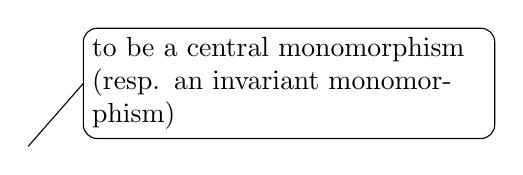
\begin{tikzpicture}
\node[align=left,text width=5cm,inner sep=3pt] (n) at (0,0) {to be a central monomorphism (resp. an invariant monomorphism)};
\draw[rounded corners=5pt] (n.south west) rectangle (n.north east);
\draw (n.west) -- ++(-.7,-.8);
\end{tikzpicture}}}}\uline{, it is necessary and sufficient that there exist $i\handwritten{\in}I$, $i\handwritten{\geqslant}j$ such that $u_i=u_j\handwritten{\times}_{S_j}S_i$ have the \inserted{\handwritten{same}}property $\deleted{\handwritten{\unsure{\mathbb{P}}}}$.}

\deleted{The assertions (i) to (iv) follow from (EGA 8.10.5). The assertions (v) and (vi) are}\inserted{\handwritten{This is}} an immediate consequence of \deleted{(EGA 8.8.2 and 8.8.3)}\inserted{\handwritten{(10.0) and (10.1),}} taking into account the characterization given in (6.7) of central and invariant group monomorphisms.

\inserted{\handwritten{\uline{Corollary}}} \uuline{10.5.} \uline{Let $j\handwritten{\in}I$, and let $G_j$ be an $S_j$-group of finite presentation. For $G=G_j\handwritten{\times}_{S_j}S$ to be abelian, it is necessary and sufficient that there exist $i\handwritten{\in}I$, $i\handwritten{\geqslant}j$, such that $G_i=G_j\handwritten{\times}_{S_j}\deleted{\unsure{H}_{\unsure{j|i}}}\inserted{S_i}$ be abelian.}

Indeed, it amounts to the same to say that an $S$-group is abelian, or that, considered as a subgroup prescheme of itself, it is central.

\uline{Proposition 10.6.}- \uline{In the s\unsure{i|à}tuation recalled at the beginning of (10.0), let $j\handwritten{\in}I$, $G_j$ be an $S_j$-group of finite presentation, $G'_j$ a subgroup prescheme of $G_j$ flat and of finite presentation over $S_j$. For $G_j\handwritten{\times}_{S_j}S/G'_j\handwritten{\times}_{S_j}S$ to be representable (for the fpqc topology), it is necessary and sufficient that there exist $i\handwritten{\in}I$, $i\handwritten{\geqslant}j$, such that $G_j\handwritten{\times}_{S_j}S_i/G'_j\handwritten{\times}_{S_j}S_i$ be representable.}

This is a consequence \deleted{p}of the following more general lemma :

\margin{\handwritten{$\mathbb{T}$}}
\uline{Lemma 10.7.}- \uline{Let $\handwritten{\mathbb{T}}$ be the fppf or fpqc topology; let $j\handwritten{\in}I$, $X_j$ be an $S_j$-prescheme of}
